\documentclass[12pt,a4paper]{article}

\usepackage[utf8]{inputenc}
\usepackage[greek,english]{babel}
\usepackage{float}
\usepackage[export]{adjustbox}
\usepackage{sans}
\usepackage{kerkis} 
%\usepackage{sans}
%\usepackage[LGRgreek]{mathastext}   
\usepackage{graphicx}
\usepackage{enumerate}
%\usepackage{enumitem}  
\usepackage{amsmath}
\usepackage{hyperref,xcolor} 
\usepackage{subcaption}

\hypersetup{
    colorlinks,
    linkcolor={black!50!black},
    citecolor={blue!50!black}, urlcolor={cyan!80!black},
}

\newcommand{\en}{\selectlanguage{english}} 
\newcommand{\tl}{\textlatin} 
\newcommand{\gr}{\selectlanguage{greek}}   
\newcommand{\code}[1]{\texttt{#1}}         
%\newcommand{\tsuper}{\textsuperscript} \newcommand{\tsub}{\textsubscript}
\renewcommand{\labelenumi}{\alph{enumi}}

 \renewcommand{\thesection}{\arabic{section}.} 
% \renewcommand{\thesubsection}{\arabic{subsection}.}


\gr \title{{\bf 
\includegraphics[scale=1.0]{images/up_landscape.jpg} \\ ΤΜΗΜΑ ΜΗΧΑΝΙΚΩΝ ΗΛΕΚΤΡΟΝΙΚΩΝ ΥΠΟΛΟΓΙΣΤΩΝ ΚΑΙ ΠΛΗΡΟΦΟΡΙΚΗΣ  \\ \vspace{3cm}Αναφορά Εργαστηριακής Άσκησης Μέρος Α' \\ Υπολογιστική Νοημοσύνη}}
\author{Κωνσταντίνος Τσάκωνας \\ Α.Μ.: 1059666}
\date{Ακαδημαϊκό έτος 2020-21\\ Χειμερινό Εξάμηνο}

\begin{document}

    \gr \maketitle \newpage

    \tableofcontents  \newpage

    \section{\tl{Repository} \gr Κώδικα}
        \underline{\tl{\textbf{\url{https://github.com/iamtsac/computational-intelligence-part-a}}}}

    \section{Προεπεξεργασία και Προετοιμασία δεδομένων.} 
    \begin{enumerate}
        \item 
        Το σύνολο των δεδομένων μας αποτελείται από $785$ στήλες. Στην πρώτη στήλη του αρχείου \tl{csv} ο περιέχεται αριθμός που απεικονίζεται στην εικόνα, ο οποίος είναι το  \tl{label} για το νευρωνικό. Οι υπόλοιπες στήλες αποτελούν τα \tl{pixels} της εικόνας. Οπότε το νευρωνικό μας θα έχει ως είσοδο τις στήλες που περιέχουν τα \tl{pixels} και θα εκπαιδευτεί στα δεδομένα του \tl{label}. Στο κώδικα εργαζόμαστε ως εξής, αφού φορτώσουμε τα δεδομένα του \tl{csv(train\_csv)} χρησιμοποιώντας το pandas, χωρίζουμε το \tl{y(label)} από το \tl{x(pixels)}. Στη συνέχεια μετασχηματίζουμε τη λίστα της εισόδου σε ένα ώστε να περιέχει $60.000$ μητρώα $28\times28$ διαστάσεων. Τη παραπάνω εργασία εφαρμόζουμε και στα δεδομένα που έχουμε για τον έλεγχο(\tl{train\_csv}). Μέτα από τα παραπάνω θα προκύψει μια δομή δεδομένων \tl{np.array} διαστάσεων ($6000,28,28$) όπου κάθε θέση θα περιέχει στοιχεία της μορφής:
        \begin{equation*}
        X_i = 
        \begin{bmatrix}
            pixel_{1,1} & pixel_{1,2} & \cdots & pixel_{1,28} \\
            pixel_{2,1} & pixel_{2,2} & \cdots & pixel_{2,28} \\
            \vdots      & \vdots      & \ddots & \vdots  \\
            pixel_{28,1} & pixel_{28,2} & \cdots & pixel_{28,28} 
        \end{bmatrix} 
        \end{equation*}
        \item Για το συγκεκριμένο ερώτημα χωρίσαμε τα $60000$ δείγματα σε $5$ κομμάτια. Αφού έγινε ο διαχωρισμός παίρνουμε το κάθε κομμάτι που προκύπτει από την διάσπαση και κάνουμε επικύρωση με τα υπόλοιπα. Ουσιαστικά χρησιμοποιώντας μία επανάληψη είχαμε σε κάθε εκπαίδευση του μοντέλου $48000$ δεδομένα εκπαίδευσης και $12000$ δεδομένα επικύρωσης. Με αυτό το τρόπο δίνουμε εκπαιδεύουμε το μοντέλο μας σε δεδομένα που δεν έχει ξαναδεί. Κατά αυτόν τον τρόπο μπορούμε να αξιολογήσουμε πως θα ανταποκριθεί το μοντέλο μας σε πραγματικές συνθήκες και μπορούμε επίσης σε περίπτωση που έχουμε να επιλέξουμε μεταξύ αρχιτεκτονικών να συγκρίνουμε τα αποτελέσματα τους από το \tl{Cross-Validation } και να διαλέξουμε την καλύτερη.
    \end{enumerate}

    \section{Επιλογή Αρχιτεκτονικής.}

    \begin{enumerate}[a]
        \item Στο συγκεκριμένο πρόβλημα μπορούμε να αξιολογήσουμε το μοντέλο μας κάνοντας χρήση του \tl{Cross-Entropy} ή του \tl{Mean-Squared-Error}. Το \tl{MSE} αυτό που μας δείχνει για το μοντέλο μας είναι, ότι όσο μικραίνει το \tl{MSE} τόσο πιο κοντά είναι η έξοδο μας στο επιθυμητό αποτέλεσμα. Από την άλλη το \tl{CE} χρησιμοποιείται για να κατηγοριοποιήσει το δεδομένα σε κλάσεις. Θα μπορούσε το  \tl{Cross-Entropy} να ερμηνευθεί ως η πιθανότητα να ανήκει η έξοδο του μοντέλου μας σε κάποια κλάση. Στη περίπτωση μας το \tl{CE} είναι πιο ιδανικό αφού θέλουμε αφού αυτό που εμείς θέλουμε είναι να κατηγοριοποιήσουμε την είσοδο μας σε μία κατηγορία από τις $[0 $-$ 9]$.

        \item Το νευρωνικό μας θα έχει πλήθος εισόδων $ 28^2 = 784 $ δηλαδή όσα είναι και  τα \tl{pixels} σε κάθε εικόνα. Ουσιαστικά με αυτό τον τρόπο δίνουμε στο μοντέλο μας σαν είσοδο μία εικόνα και προσπαθεί να κατηγοριοποιήσει σε μια κλάση. 

        \item Στην έξοδο θα χρειαστούμε 10 νευρώνες.  Αυτό συμβαίνει γιατί θέλουμε η έξοδος του νευρωνικού μας να καθορίζει την κλάση που ανήκει η εικόνα που δώσαμε σαν είσοδο.

        \item Στους κρυφούς κόμβους η συνάρτηση ενεργοποίησης που διαλέξαμε είναι η \tl{ReLU}. Η απόφαση για την συνάρτηση του κρυφού επιπέδου είναι αρκετά εύκολη, αρκεί να παρατηρήσουμε την γραφική παράσταση της συνάρτηση και το είδος των δεδομένων. Τα δεδομένα μας είναι εικόνες, από \tl{pixels} οι τιμές των οποίων μετά τη κανονικοποίηση κυμαίνονται στο διάστημα $[0,1]$. Ο τύπος της συνάρτησης \tl{ReLU} είναι ο εξής: 
        $$ f(x)=\max(0,x)$$ 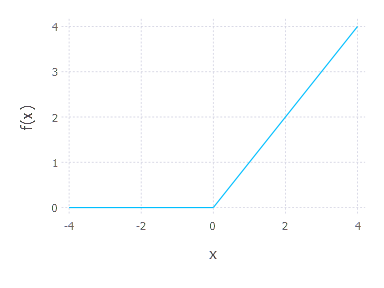
\includegraphics[ height=6cm, center]{images/relu_graph.png} \\ 
        Χρησιμοποιώντας τη \tl{ReLU} πετυχαίνουμε αρκετά πράγματα εξαιτίας της φύσης του συνόλου δεδομένων που έχουμε. Αρχικά τα δεδομένα είναι αρκετά αραιά, οπότε για κάθε είσοδο δεν θα ενεργοποιούνται όλοι οι νευρώνες, με αποτέλεσμα οι τιμές που δεν προσφέρουν κάποια πληροφορία στο νευρωνικό να μην επηρεάζουν την εκπαίδευση. Επίσης τα μητρώα έχουν τις τιμές που μας ενδιαφέρουν κοντά στο κέντρο, οπότε κατά την πρόοδο της εκπαίδευση θα δούμε μεγάλη βελτίωση αφού θα είναι αρκετά εύκολο για το νευρωνικό να τοποθετήσει τα σωστά βάρη στους κόμβους. Τέλος προσφέρει πολύ μικρή υπολογιστική πολυπλοκότητα στο δίκτυο μας, αφού το μόνο που κάνει είναι απλά μία σύγκριση. 

        \item Στο επίπεδο εξόδου θα χρησιμοποιήσουμε την συνάρτηση \tl{Softmax}, διότι συναρτήσεις όπως  η σιγμοειδής δεν μπορεί να μας βοηθήσει σε ένα πρόβλημα κατηγοριοποίησης σε περισσότερες από δύο κλάσεις όπως αυτό που έχουμε εδώ.  Αυτό που κάνει η \tl{Softmax} και μας είναι απαραίτητο στο συγκεκριμένο πρόβλημα είναι ότι στη έξοδο συμπυκνώνει τις τιμές μεταξύ του διαστήματος $[0,1]$ και το άθροισμα των εξόδων ισούται με $1$. Άρα πρακτικά η συνάρτηση μας δίνει σαν έξοδο την πιθανότητα να ανήκει η είσοδος μας σε κάθε κατηγορία.

        \item Για τα παρακάτω αποτελέσματα χρησιμοποιήθηκαν 30 εποχές εκπαίδευση.

            \begin{tabular}{|c | c | c | }
                \hline
                Αριθμός νευρώνων στο κρυφό επίπεδο & \tl{CE loss} & \tl{MSE} \\
                \hline
                $H_1 = O$       & 0,487 & 0,087 \\ 
                $H_1 = (I+O)/2$ & 0,385 & 0,0832 \\ 
                $H_1 = I+O$     & 0,378 & 0,0833 \\
                \hline 
            \end{tabular} \\
            
            Παρακάτω φαίνονται οι γραφικές παραστάσεις: 
            \begin{figure}[H]
                \raggedright
                    \begin{subfigure}[t]{0.5\textwidth}
                        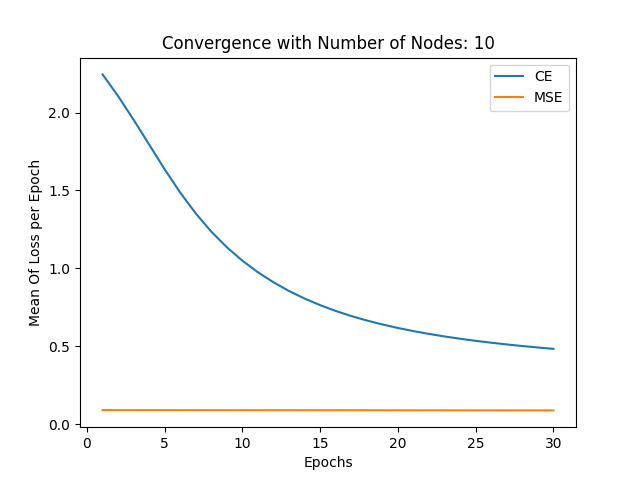
\includegraphics[width=10cm,height=7cm,left]{images/10.png}
                    \end{subfigure}
                    \begin{subfigure}[t]{0.5\textwidth}
                        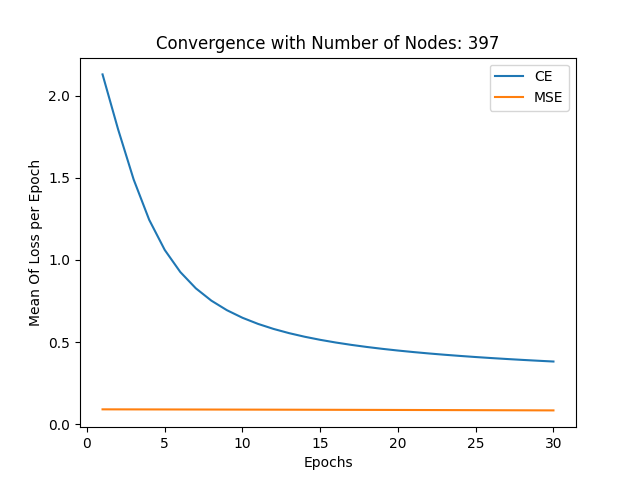
\includegraphics[width=10cm,height=7cm,left]{images/397.png} 
                    \end{subfigure}
                    \begin{subfigure}[t]{0.5\textwidth}
                        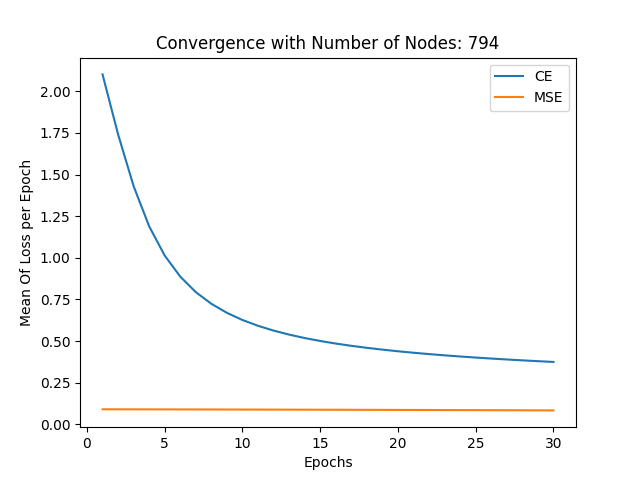
\includegraphics[width=10cm,height=7cm,left]{images/794.png} 
                    \end{subfigure}
            \end{figure}

            \begin{enumerate}[i)]
                \item  Από τα παραπάνω αποτελέσματα παρατηρούμε ότι η εκπαίδευση που είχε πλήθος κρυφών κόμβων ίσο με τον αριθμό των εξόδων παρουσίασε μεγαλύτερο λάθος. Οι υπόλοιπες δύο μετρήσεις είχαν πλήθος κόμβων αρκετά μεγαλύτερο του αριθμού των εξόδων και παρατηρούμε ότι το λάθος σε αυτές τις μετρήσεις είναι μικρότερο. Το οποίο είναι αναμενόμενο αφού όσους περισσότερους κόμβους έχουμε στο κρυφό επίπεδο τόσο πιο πολύπλοκο θα είναι το νευρωνικό μας δίκτυο με αποτέλεσμα να έχει καλύτερη ακρίβεια. Ένας σημαντικός παράγοντας όμως είναι και ο χρόνος που χρειάστηκε να εκπαιδευτεί το νευρωνικό μας. Περισσότερων χρόνο κατανάλωσαν το νευρωνικό που είχε $794$ κρυφούς κόμβους, οπότε βέλτιστος αριθμός κόμβος είναι $H_1 = 397$ αφού η διαφορά στο \tl{loss} είναι ελάχιστη αλλά η ταχύτητα εκπαίδευσης σαφώς μεγαλύτερη.
                \item Εστιάζοντας στη συνάρτηση κόστους κάποιος θα μπορούσε να πει ότι με βάση \tl{MSE} το νευρωνικό μας κάνει πολύ σπάνια λάθος, πράγμα που δεν είναι σωστό. Διότι παρατηρήθηκε ότι ναι μεν η συνάρτηση κόστους \tl{MSE}  μπορεί να δείχνει ότι το λάθος του νευρωνικού μας είναι σχεδόν μηδενικό αλλά η ακρίβεια του ήταν κάκιστη. Το αποτέλεσμα αυτό ήταν αρκετά προβλέψιμο αφού το η συνάρτηση κόστους \tl{MSE}  δεν είναι η κατάλληλη συνάρτηση για προβλήματα ταξινόμησης σε κλάσεις αφού δεν "τιμωρεί" σωστά τις λάθος ταξινομήσεις. Από την άλλη η συνάρτηση κόστους \tl{CE} αντικατοπτρίζει την πραγματικότητα της απόδοσης του νευρωνικού μας αφού η λειτουργία της απευθύνεται σε προβλήματα ταξινόμησης όπως το δικό μας. Ο λόγος που καθιστά την \tl{CE} καταλληλότερη από την \tl{MSE} αναφέρεται παραπάνω στο ερώτημα Α3.α.
                \item Παρατηρώντας τις γραφικές παραστάσεις βλέπουμε ότι τις πρώτες 10 εποχές η ταχύτητα σύγκλισης είναι μεγαλύτερη από τις υπόλοιπες. Αυτό συμβαίνει διότι αρχικά το νευρωνικό μας δεν έχει τοποθετήσει κάποια βάρη στους νευρώνες. Με αποτέλεσμα αρχικά να κάνει αρκετά λάθη αλλά καθώς επέρχονται οι εποχές και μετά από τις συνεχείς διορθώσεις βαρών φθάνει σε κάποιο σημείο όπου οι μεταβολές στα βάρη είναι μικρότερες, για αυτό και παρατηρούμε την καμπύλη στις τελευταίες εποχές να μεταβάλλεται ελάχιστα.
            \end{enumerate}

        \item Αρχικά πρέπει να ορίσουμε το καινούργιο κρυφό επίπεδο και τη συνάρτηση ενεργοποίησής τους. Αρχικά στο μοντέλο μας προσθέσαμε ένα πλήρης διασυνδεδεμένο δίκτυο ( \tl{Dense} ) και στη συνέχεια πειραματιστήκαμε με την συνάρτηση ενεργοποίησής. Οι συναρτήσεις που δοκιμάστηκαν ήταν οι \tl{tanh, Sigmoid} και \tl{ReLU }. Από αυτές η \tl{Sigmoid} είχε την χειρότερη χειρότερη απόδοση με λάθος που έφτανε κοντά στο 0,6. Η \tl{tanh} είχε λίγο χειρότερη απόδοση από την \tl{ReLU}, οπότε καταλήξαμε να χρησιμοποιήσουμε την \tl{ReLU}. Το τελευταίο κομμάτι που απομένει για το δεύτερο κρυφό επίπεδο είναι να καθορίσουμε τον αριθμό των κόμβων. Έχοντας δοκιμάσει αρκετά πλήθη κόμβων, βάση απόδοσης καταλήξαμε στο αριθμό $128$, που είχε την καλύτερη απόδοση, παρόλα αυτά η διαφορά στην απόδοση μεταξύ του πλήθους των κόμβων ήταν ελάχιστη αλλά επίσης παρατηρείται ότι δεν υπάρχει κάποια τεράστια βελτίωση από το προηγούμενο ερώτημα που είχαμε ένα κρυφό επίπεδο. Ο λόγος που οφείλεται αυτό έχει να κάνει και με την φύση του \tl{dataset} το οποίο είναι αρκετά \tl{optimized} για τη δημιουργία ενός μοντέλου που κάνει \tl{classification}. Τέλος δεν υπάρχει κάποιος γενικός κανόνας για το πως καθορίζεται ο αριθμός των κόμβων, αλλά γενικά μπορούμε να πούμε ότι πρέπει ο αριθμός αυτός να είναι μικρότερος από το πλήθος των εισόδων και μεγαλύτερος από το πλήθος των εξόδων, η τελική απόφαση για το πόσοι κόμβοι θα υπάρχουν προκύπτει μετά από εκτενείς πειραματισμούς. Παρακάτω παρουσιάζεται ο πίνακας με τα αποτελέσματα των σ κόστους μερικών από των πειραμάτων που έγιναν. \\ 

            \begin{tabular}{|c | c | c | }
                \hline
                Αριθμός νευρώνων στο κρυφό επίπεδο & \tl{CE loss} & \tl{MSE} \\
                \hline
                $H_2 = 397$ & 0,303 & 0,086 \\ 
                $H_2 = 128$ & 0,290 & 0,085 \\ 
                $H_2 = 512$ & 0,307 & 0,086 \\
                \hline 
            \end{tabular} \\
        \item 

    \end{enumerate}

\end{document} 